\documentclass{article}
\usepackage{tikz, comment}
\usepackage{pifont}
\usepackage{fontspec, pgfplots}
\usetikzlibrary{arrows, decorations.markings, decorations.pathreplacing}
\begin{comment}
:Title: Not defined yet
:Tags: x-y plane;y-z plane;area using parametric equations,parametric integral formula;x-z plane;two intercept form for the equation of a line
:Prob: 0.5195;0.5127;0.503;0.499;0.4957
:Author: Prof.Hu Ji-shan, HKUST
:Slug: No name yet

Description Here.........
\end{comment}
\begin{document}\centering 

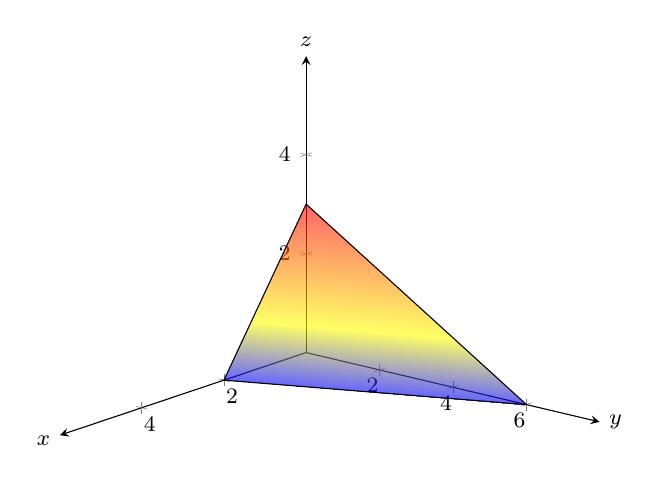
\begin{tikzpicture}[font=\footnotesize]
\pgfplotsset{compat=1.8}
\begin{axis}
[axis lines = center, view={130}{20},
axis background, xlabel = {$x$}, ylabel ={$y$}, zlabel ={$z$}, domain =-2:2, y domain =-2:2,
xmin =0,
xmax =5.99,
ymin =0,
ymax =7.99,
zmin =0, 
zmax =5.99,
samples =10, samples y =40, z buffer = auto, 
every axis x label/.style={
    at={(ticklabel* cs:1)},
    anchor= east, yshift =-2
},
every axis y label/.style={
    at={(ticklabel* cs:1)},
    anchor= west,
},
every axis z label/.style={
    at={(ticklabel* cs:1)},
    anchor= south
}]

\addplot3[surf, shader=interp, mesh/cols=2, opacity=0.6] coordinates
		{(2,0,0) (0,6,0) (0,0,3) (0,0,3)};

\addplot3[surf, black] coordinates
		{(2,0,0) (0,6,0)};
\addplot3[surf, black] coordinates
		{(0,0,3) (0,6,0)};	
\addplot3[surf, black] coordinates
		{ (0,0,3) (2,0,0)};	
		 
\end{axis}

\end{tikzpicture}
\end{document}